\chapter{Threads and Services}
\label{TAS}

\section{Introduction}
\label{TAS:introduction}
--- To be filled ---

\section{Threads}
\label{TAS:threads}
Before anything else let's first create a fresh project.

\subsection{Create New Project}
\label{TAS:createNewProject1}
Close any open projects and create a new project as follows:
\begin{enumerate}
	\item Create a new project having name ``\texttt{Threads App}''.
	\item Select minimum API 16 : Android 4.1 (Jelly Bean).
	\item Select ``\texttt{Empty Activity}''
	\item \textbf{Important:} At the final dialog box ``\underline{uncheck}'' backwards compatibility option. Accept other values as hit finish.
	
	\begin{center}
		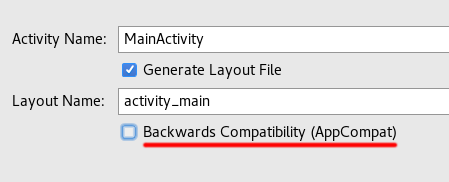
\includegraphics[scale=\SourceCodeScale]{chapters/ch14/images/1}
	\end{center}
	
	Run the project on a device and make sure it is working properly.
\end{enumerate}	

\subsection{UI Thread Model}
\label{TAS:uiThreadModel}
By default the android operating system executes an activity on a ``main'' thread (also known as the ``UI'' thread). All of the code, buttons, messages etc execute on this ``UI'' thread. Sometimes you need to perform heavy operations that could block the UI thread resulting in the famous \href{https://developer.android.com/training/articles/perf-anr.html}{ANR} dialog. Aditionally the android user interface widgets are NOT thread safe. This means that they need to be accessed from WITHIN the UI thread. If an outside thread tries to access these it will result in unexpected behavior. 

To make high quality responsive apps following two rules must be followed:

\begin{enumerate}
	\item Do not block the main UI thread. It is recommended to run the heavy computations in a separate thread. 
	\item Never access UI toolkit from outside the main UI thread. For this there are multiple solutions.
\end{enumerate}

Let's first see the basic worker thread in action.

\subsection{Worker Thread}
\label{TAS:workerThread}
Open up \texttt{activity\_main.xml} and create a basic layout as follows (a text view, a button):

\begin{center}
	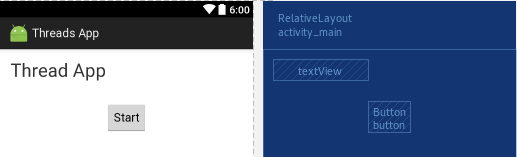
\includegraphics[scale=\FigureScale]{chapters/ch14/images/18}
\end{center}

Now open up \texttt{MainActivity} and modify it as follows:

\begin{center}
	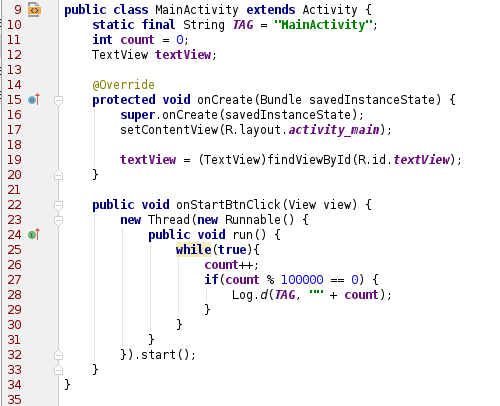
\includegraphics[scale=\SourceCodeScale]{chapters/ch14/images/19}
\end{center}

Code explanation:
\begin{itemize}
	\item \textit{Lines 11:} Create an integer member variable that we will use shortly.
	
	\item \textit{Lines 12:} Variable to hold reference to the text view object.
	
	\item \textit{Lines 19:} Get the reference to the text view object.
	
	\item \textit{Lines 23:} Inside the \texttt{onStartBtnClick} event listener we are creating a new thread. How do we specify the code to run by this thread? Through the \href{https://developer.android.com/reference/java/lang/Runnable.html}{\texttt{Runnable}} interface. Here \texttt{Runnable} is acting as an anonymous inner class.
	
	\item \textit{Lines 24:} \texttt{Runnable} interface has got exactly one abstract method named \texttt{Run} which should be implemented. The \texttt{Run} method contains code to be run in the new thread. Pretty simple !!!
	
	\item \textit{Lines 25 to 30:} An infinite while loop that keeps on printing log messages in the logcat window. You can potentially write ANY imaginable code in inside the \texttt{Run} method.
	
\end{itemize}

Open up the android studio's logcat window and run the app. Click the start button and you should see log messages in the logcat window being printed like crazy. The interesting thing to note is that this infinite loop has not blocked the UI thread because it is running in a separate thread. \\

Let's say that we want the text view to display the updated value of \texttt{counter}. Our natural reaction would be to go to the thread code and update the text view widget right there as follows i.e: change line 28 from \texttt{Log.d} to \texttt{textView.setText}:

\begin{center}
	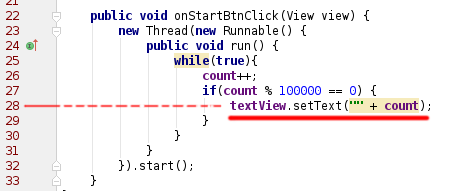
\includegraphics[scale=\SourceCodeScale]{chapters/ch14/images/20}
\end{center}

Seems logical and it should work. Run the app on a device, press the start button and watch it crash !! Why did this happen? Recall that we mentioned two rules. Here are violated the second rule. We are modifying UI toolkit outside the UI thread. To simply put we must change the text view within the main thread and NOT inside the new thread. But how will be update the text view? There are a few solutions available as mentioned \href{https://developer.android.com/guide/components/processes-and-threads.html#WorkerThreads}{here} but we will use \href{https://developer.android.com/reference/android/view/View.html#post(java.lang.Runnable)}{\texttt{View.post(Runnable)}}. Delete the above line and replace it with the following code:

\begin{center}
	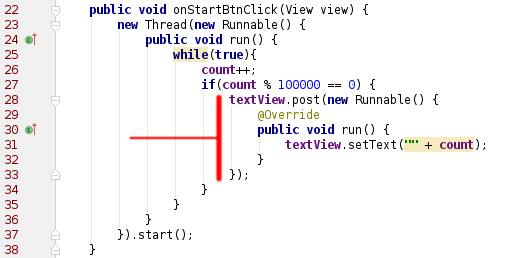
\includegraphics[scale=\SourceCodeScale]{chapters/ch14/images/21}
\end{center}

Let's analyze the code:

\begin{itemize}
	\item \textit{Line 28:} Every \href{https://developer.android.com/reference/android/view/View.html}{\texttt{View}} has a method named \href{https://developer.android.com/reference/android/view/View.html#post(java.lang.Runnable)}{\texttt{post}}. This method delays the execution of a piece of code untill it is back in the UI thread again. 
	
	\item \textit{Line 30:} Here we are giving it the code that will be run OUTSIDE the new thread. \texttt{View}'s post method will add this to a message queue and it will run only when in the main UI thread.
	
	\item \textit{Line 31:} We are delaying the update to the text view until it is back in the UI thread.
	
\end{itemize}

Run the app now and press start button. Watch how the text view is updated with the current value of the counter. How beautiful !!!

\begin{quote}
	\textit{``Note: You can use the post method with any UI widgets so that they are updated only in the main UI thread''.}
\end{quote}

\subsection{Asynchronous Task}
\label{TAS:asyncTask}
\href{https://developer.android.com/reference/android/os/AsyncTask.html}{\texttt{AsyncTask}} is a special type of thread that performs work and then automatically updates the UI inside main UI thread. How cool is that !!!

You can read more about asynchronous tasks \href{https://developer.android.com/reference/android/os/AsyncTask.html}{here}.

\subsubsection{Exercise}
Read more about \href{https://developer.android.com/reference/android/os/AsyncTask.html}{\texttt{AsyncTask}}. Modify the above example from section \ref{TAS:workerThread} and replace traditional threads with \texttt{AsyncTask} such that the app still runs exactly as before. There should be no visible difference to the user.

\section{Services}
\label{TAS:services}
Before anything else let's first create a fresh project.

\subsection{Create New Project}
\label{TAS:createNewProject}
Close any open projects and create a new project as follows:
\begin{enumerate}
	\item Create a new project having name ``\texttt{Services App}''.
	\item Select minimum API 16 : Android 4.1 (Jelly Bean).
	\item Select ``\texttt{Empty Activity}''
	\item At the final dialog box ``\underline{uncheck}'' backwards compatibility option. Accept other values as hit finish.
\end{enumerate}	

\subsection{Basics}
\label{TAS:basics}
A \href{https://developer.android.com/guide/components/services.html}{\texttt{Service}} is a component that runs in the background, it has no user interface. Services are useful when you want to download something or listen to social media status update or play songs in the background or update lots of records in a database etc, the possibilities are limitless. 

There are three types of services: scheduled, started and bound. Let's discuss these one by one.

\subsection{Scheduled Services}
\label{TAS:scheduledServices}
These services are scheduled to run after a specified time interval. Usually a \href{https://developer.android.com/reference/android/app/job/JobScheduler.html}{\texttt{JobScheduler}} will be responsible for scheduling services.

We won't be discussing these types of services in detail in this book. But you can check out more information \href{URL}{here}.

\subsection{Started Services}
\label{TAS:startedServices}
These types of services perform a single task. They can potentially run indefinitely even if the starting app or activity has been terminated. 

\textit{``It is the service's responsibility to destroy itself cleanly after it has finished it's job. This type of service does not communicate with or return any result to the starting activity.''}

\subsubsection{Create a New Service}
\label{TAS:createNewService}
As mentioned earlier that a service runs in the background and has no user interface. In order to create a service you need a java file and add an entry in the android manifest file. There is no need to create a layout file like we did when creating activities.

\href{URL}{\texttt{IntentService}} is a subclass of \href{URL}{\texttt{Service}} that implements some convenience features. Also unlike \texttt{Service}, \texttt{IntentService} runs in a ``separate thread'' but in the same process as the starting activity. We will extend our services from \texttt{Service} class in section \ref{TAS:boundServices} where we create bounded services.

Create a new \texttt{java} class and name it ``\texttt{StartedService}''. Make sure that it is in the same folder as the \texttt{MainActivity}:

\begin{center}
	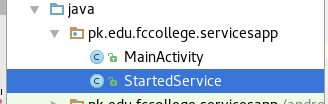
\includegraphics[scale=\SourceCodeScale]{chapters/ch14/images/2}
\end{center}

Open up ``\texttt{StartedService.java}'' and extend \texttt{StartedService} class from the ``\texttt{IntentService}'':

\begin{center}
	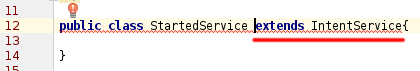
\includegraphics[scale=\SourceCodeScale]{chapters/ch14/images/3}
\end{center}

You will see errors because ``\texttt{IntentService}'' is an abstract class and you must implement its ``\texttt{onHandleIntent}'' method. Also don't forget to implement a default constructor:

\begin{center}
	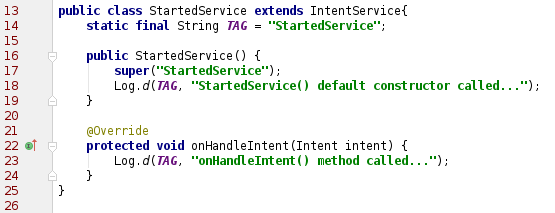
\includegraphics[scale=\SourceCodeScale]{chapters/ch14/images/4}
\end{center}

Let's analyze the above code line by line:

\begin{itemize}
	\item \textit{Line 14:} Declare a \texttt{TAG} member variable so that we don't have to manually type it in every log commands.

	\item \textit{Lines 16 to 19:} You MUST provide a default constructor for every service that you implement. Also you need to call the constructor for super class and pass it the name of the service, as done in line 17.

	\item \textit{Lines 22 to 24:} You must implement \texttt{onHandleIntent} method. This is the method which performs the actual tasks of the service. You can put virtually anything here, upload pictures, download movies, modify databases etc. This method gets called as soon as an activity starts the service. As soon as this method exits and if no other activity has requested it then the service is terminated. 
	
	Here we are just displaying a simple log message to keep things simple.

\end{itemize}

That is pretty much it. Above is a fully functional service. Before you can use it you need to define it in the manifest file. \\

Open up \texttt{AndroidManifest.xml} and add a \texttt{<service>} within the \texttt{<application>} but outside \texttt{<activity>} tags (lines 19 to 21):

\begin{center}
	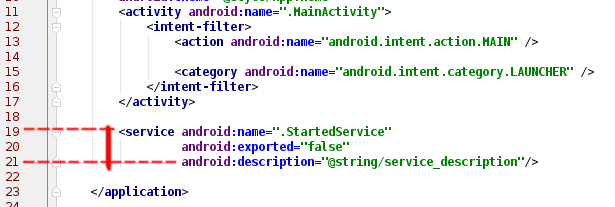
\includegraphics[scale=\SourceCodeScale]{chapters/ch14/images/5}
\end{center}

XML code explaination:
\begin{itemize}
	\item \textit{Line 19:} Define a service in the manifest file. The only \textit{required} parameter when defining a service is the ``\texttt{name}''. Here you give the exact name of the service class that you are creating. Note that the name is beginning with a ``\texttt{.}''. This is a short hand form so that you don't have to type the entire package name before the class name.
	
	\item \textit{Line 20:} This is an \textit{optional} parameter. When you set \texttt{exported} to \texttt{false} then only the activities in the current package will be able to use it. Other activities belonging to other apps will NOT be able to use or even this service.
	
	\item \textit{Line 21:} Another \textit{optional} parameter. It is always a good idea to set the description of your service which the user can see when he in his list of running apps and services.
\end{itemize}

Now open up \texttt{activity\_main.xml} and make a very simple layout as follows. It has one text view and two buttons:

\begin{center}
	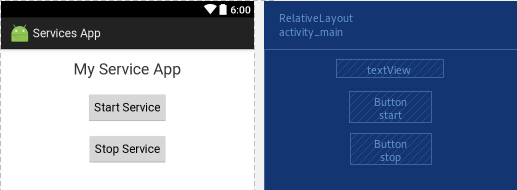
\includegraphics[scale=\SourceCodeScale]{chapters/ch14/images/6}
\end{center}

Add click listeners to these buttons in the \texttt{MainActivity} class (your method names can be different). In the service start button listener add code to start our service:

\begin{center}
	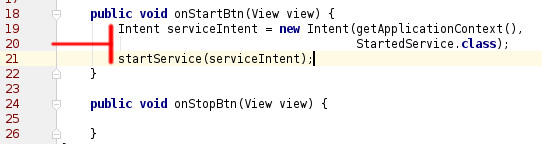
\includegraphics[scale=\SourceCodeScale]{chapters/ch14/images/7}
\end{center}

Code explanation:
\begin{itemize}
	\item \textit{Lines 19 to 21:} This code should look very familiar. We are first creating an explicit intent. Then we are starting a service by calling the ``\texttt{startService}'' method. 
\end{itemize}

Run the app on a device and as soon as you click the start service button following logs will be displayed in the logcat window:

\begin{center}
	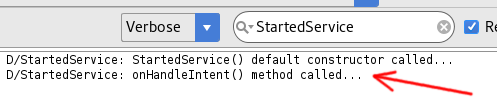
\includegraphics[scale=\SourceCodeScale]{chapters/ch14/images/8}
\end{center}

\subsection{Service Lifecycle}
\label{TAS:serviceLifecycle}
Just like an activity, a service also undergoes through a series of lifecycle events \textit{independently} of the calling activity. Unlike an activity the service lifecycle is very simple and there are only a handful of events as shown in the figure below:

\begin{center}
	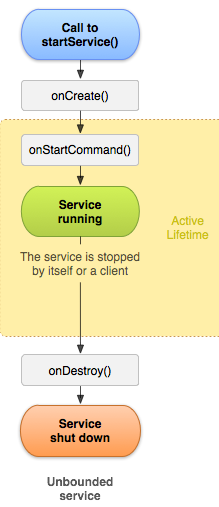
\includegraphics[scale=\FigureScale]{chapters/ch14/images/9}
\end{center}

Note that the above lifecycle diagram is for ``started services''. For bound services the lifecycle differs slightly. \\

Open up \texttt{StartedService.java} file and implement the life cycle methods as follows:

\begin{center}
	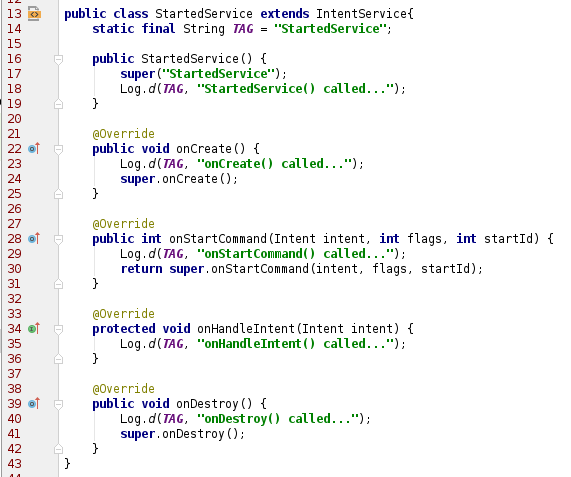
\includegraphics[scale=\SourceCodeScale]{chapters/ch14/images/10}
\end{center}

These should look familiar. As with activity lifecycles, in each of the  service lifecycle methods you need to call the super class variants. The green box shown in the service lifecycle above is actually the \texttt{onHandleIntent} method where all the action is taking place. 

\begin{quote}
	\textit{``Note that when implementing an \texttt{IntentService} you should \textbf{NOT} override the \texttt{onStartCommand} method. All of the task implementation code should reside in \texttt{onHandleIntent}.''}
\end{quote}

When you run the app on a device and press ``start service'' button you should see the following output in the logcat window:

\begin{center}
	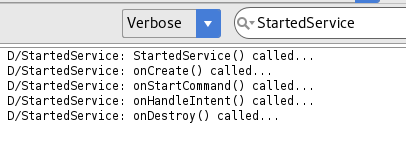
\includegraphics[scale=\SourceCodeScale]{chapters/ch14/images/11}
\end{center}

The call to \texttt{startService} initiated the service. As you can see all the lifecycle methods were called in correct order. \\

Let's make the app a little bit more complex. Open up \texttt{StartedService.java}. Modify the \texttt{onHandleIntent} method as follows:

\begin{center}
	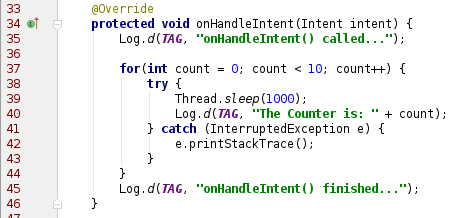
\includegraphics[scale=\SourceCodeScale]{chapters/ch14/images/12}
\end{center}

The above code is very simple. It is counting up to 10, displaying each number in the logcat window after every second. When the loop terminates and the \texttt{onHandleIntent} method finishes the service is also destroyed and removed from the memory. Run the app and see if it produces expected output in the logcat window.

\begin{quote}
	\textit{``Even if you minimize the current app and switch to a different app you will still see the messages being output in the logcat window.''}
\end{quote}


\subsection{Stopping a Service}
\label{TAS:stoppingService}
Recall that an unbound or started service is responsible for destroying itself. Other activities can however ``request'' the service to stop and cleanly remove itself from the memory. \\

Open up \texttt{MainActivity.java} and add following code to the stop service button event listener:

\begin{center}
	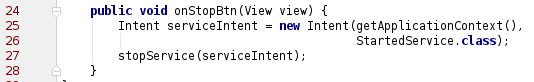
\includegraphics[scale=\SourceCodeScale]{chapters/ch14/images/13}
\end{center}

Here we are creating a new intent and passing that to \texttt{stopService} method. It the service is already running then its \texttt{onDestroy} method is called. The service should take note and stop all its running operations and terminate gracefully.\\

Open up \texttt{StartedService.java} and add a member variable named ``\texttt{boolean isDestroyed = false}'' to the \texttt{StartedService} class. Next in the \texttt{onDestroy} method set this variable to \texttt{true} so that all of the class methods may know when an activity destruction is requested:

\begin{center}
	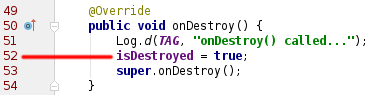
\includegraphics[scale=\SourceCodeScale]{chapters/ch14/images/14}
\end{center}

Finally go to \texttt{onHandleIntent} method and add the following condition to terminate the working loop as soon as activity is destroyed:

\begin{center}
	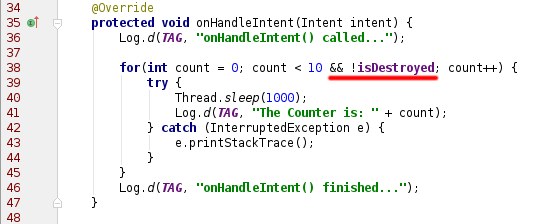
\includegraphics[scale=\SourceCodeScale]{chapters/ch14/images/15}
\end{center}

\subsection{The Intent Queue}
\label{TAS:intentQueue}
Let's perform an experiment. Open up logcat window. Run the app and press start service button. You should see lifecycle methods being called and then counter starts to display. While the counter is being run press ``start service'' exactly two times. You will see \texttt{onStartCommand} being called twice right in the middle of current output. Note that other lifecycle methods are not called (yet). 

\begin{center}
	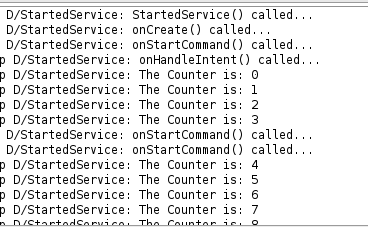
\includegraphics[scale=\SourceCodeScale]{chapters/ch14/images/16}
\end{center}

After the counter is exhausted and the \texttt{onHandleIntent} method exits the task is started again and counter starts to display from scratch. Once it finishes the \texttt{onHandleIntent} method runs for the third time displaying the counter. Finally when it finishes this time other lifecycle methods are called and the activity is destroyed. So we might ask what's going on over here?

Actually it is simpler than it looks. Whenever an intent calls a service the service puts it in an ``intent queue''. This queue contains the list of all intents that requested this service. The service removes an intent and executes \texttt{onHandleIntent} method for it. Once this method is finished AFTER THAT the service removes another intent from the queue and runs \texttt{onHandleIntent} for that. When one intent is being served all others are waiting in the queue. When the queue is empty the service is destroyed. Following figure shows a clearer picture:

\begin{center}
	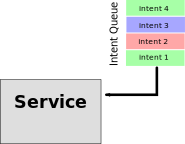
\includegraphics[scale=0.8]{chapters/ch14/images/17}
\end{center}

\begin{quote}
	\textit{``Note: No matter how many intents are present in the intent queue the service runs only on a single thread serving the intents one after another synchronously''.}
\end{quote}

\subsection{Bound Services}
\label{TAS:boundServices}
Unlike ``un-bound'' or ``started'' services that we saw in the previous sections, \href{https://developer.android.com/guide/components/bound-services.html}{bound services} can communicate with the calling activities. Since the only purpose of a bound service is to fulfill the requirements of the attached activity or a component it lives only as long as the calling activity. You can not start an bound service using \texttt{startService}. As a consequence unlike started service a bound service can not run indefinitely. \\

-- Advanced topic. Under construction --

\subsection{Inter Process Communication}

-- Advanced topic. Under construction --










